\subsubsection*{Dados los siguientes requerimientos hacer el subnetting:}

\begin{itemize}
\item Red Base: \texttt{180.147.39.0/24}

\begin{table}[ht]
    \begin{tabular}{|r|c|c|c|}
        \hline
        ~           & IPs & IPs Solicitadas & IPs Necesarias \\ \hline
        OF. CENTRAL & 37  & 39              & 64             \\ 
        SUCURSAL 1  & 14  & 16              & 16             \\ 
        SUCURSAL 2  & 8   & 10              & 16             \\ 
        LOS POZOS   & 3   & 5               & 8              \\ 
        LA RAMADA   & 9   & 11              & 16             \\ 
        LA PAZ      & 70  & 72              & 128            \\ 
        COCHABAMBA  & 20  & 22              & 32             \\
        \hline
    \end{tabular}
\end{table}
$\sum_{\text{IPs Necesarias}}=280$ \\
Si calculamos las IPs que tiene esta red sería: $2^8=256$ y nuestro subneteo tiene 280 IPs Necesarias (solo contamos con 256) por lo que debemos cambiar la mascara de \texttt{/24} a \texttt{/23}.



\item Red Base: \texttt{192.168.0.0/23}

\begin{table}[ht]
    \begin{tabular}{|r|c|c|c|}
        \hline
        ~           & IPs & IPs Solicitadas & IPs Necesarias \\ \hline
        OF. CENTRAL & 28  & 30              & 32             \\ 
        SUCURSAL 1  & 29  & 31              & 32             \\ 
        SUCURSAL 2  & 40   & 42              & 64             \\ 
        LOS POZOS   & 13   & 16               & 16              \\ 
        LA RAMADA   & 9   & 16              & 16   
\\
        \hline
    \end{tabular}
\end{table}
$\sum_{\text{IPs Necesarias}}=160$\\
Si calculamos las IPs que tiene esta red sería: $2^8=512$ (esto es mas de las que tenemos $512>160$ por lo que podemos proceder sin problemas).
\begin{center}

\Tree
[.512
    \edge node[auto=right] {{\color{red}0}};
    [.256 
       \edge node[auto=right] {{\color{red}0}};
       [.128
       	\edge node[auto=right] {{\color{red}0}};
       	[.\fbox{64} ]
       	\edge node[auto=left] {{\color{red}1}};
       	[.64 
			\edge node[auto=right] {{\color{red}0}};
       		[.\fbox{32} ]
       		\edge node[auto=left] {{\color{red}1}};
       		[.\fbox{32} ]       	
       	]
       ]
       \edge node[auto=left] {1};
       [.128 
       ]
        ]
    \edge node[auto=left] {{\color{red}1}};
    [.256 
        \edge node[auto=right] {0};
        [.128
        ]
        \edge node[auto=left] {{\color{red}1}};
        [.128 
		\edge node[auto=right] {{\color{red}0}};
       	[.64 
			\edge node[auto=right] {{\color{red}0}};
       		[.32 
				\edge node[auto=right] {{\color{red}0}};
       			[.\fbox{16} ]
       			\edge node[auto=left] {{\color{red}1}};
       			[.\fbox{16} ]           		
       		]       	
       	]
       	\edge node[auto=left] {1};
       	[.64 ]         
        ]
        ]
]
\end{center}\begin{center}

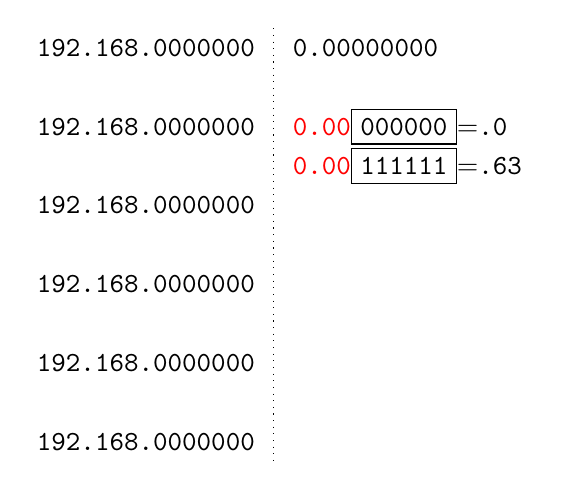
\begin{tikzpicture}
\draw[dotted] (1.5,0.25) -- (1.5,-5.25);
\node[text width=3cm] at (0,0) 
    {\texttt{192.168.0000000}};
\node[text width=3cm] at (3.25,0) 
    {\texttt{0.00000000}};
    
\node[text width=3cm] at (0,-1) 
    {\texttt{192.168.0000000}};
\node[text width=3cm] at (3.25,-1) 
    {\texttt{{\color{red}0.00}\fbox{000000}}=\texttt{.0}};
\node[text width=3cm] at (3.25,-1.5) 
    {\texttt{{\color{red}0.00}\fbox{111111}}=\texttt{.63}};

\node[text width=3cm] at (0,-2) 
    {\texttt{192.168.0000000}};
    
\node[text width=3cm] at (0,-3) 
    {\texttt{192.168.0000000}};
    
\node[text width=3cm] at (0,-4) 
    {\texttt{192.168.0000000}};
    
\node[text width=3cm] at (0,-5) 
    {\texttt{192.168.0000000}};
\end{tikzpicture}
\end{center}

\end{itemize}
